% !BIB TS-program = biber

\RequirePackage[l2tabu,orthodox]{nag}

%\documentclass[headsepline,footsepline,footinclude=false,fontsize=11pt,paper=a4,listof=totoc,bibliography=totoc,BCOR=12mm,DIV=12]{scrbook} % two-sided
\documentclass[headsepline,footsepline,footinclude=false,oneside,fontsize=11pt,paper=a4,listof=totoc,bibliography=totoc]{scrbook} % one-sided

% TODO: change citation style in settings
\PassOptionsToPackage{table,svgnames,dvipsnames}{xcolor}

\usepackage[utf8]{inputenc}
\usepackage[T1]{fontenc}
\usepackage[sc]{mathpazo}
\usepackage[ngerman,american]{babel}
\usepackage[autostyle]{csquotes}
\usepackage[%
  backend=biber,
  url=false,
  style=alphabetic,
  maxnames=4,
  minnames=3,
  maxbibnames=99,
  giveninits,
  uniquename=init]{biblatex} % adapt citation style
\usepackage{graphicx}
\usepackage{scrhack} % necessary for listings package
\usepackage{listings}
\usepackage{lstautogobble}
\usepackage{tikz}
\usepackage{pgfplots}
\usepackage{pgfplotstable}
\usepackage{booktabs}
\usepackage[final]{microtype}
\usepackage{caption}
\usepackage[printonlyused]{acronym}
\usepackage[hidelinks]{hyperref} % hidelinks removes colored boxes around references and links
\usepackage{amsmath}
\usepackage{amssymb}
\usepackage{subcaption}
\AtBeginDocument{%
	\hypersetup{
		pdftitle=\getTitle,
		pdfauthor=\getAuthor,
	}
}
\usepackage{ifthen}

\addto\extrasamerican{
	\def\lstnumberautorefname{Line}
	\def\chapterautorefname{Chapter}
	\def\sectionautorefname{Section}
	\def\subsectionautorefname{Subsection}
	\def\subsubsectionautorefname{Subsubsection}
}

\addto\extrasngerman{
	\def\lstnumberautorefname{Zeile}
}

% Themes
\ifthenelse{\equal{\detokenize{dark}}{\jobname}}{%
  % Dark theme
  \newcommand{\bg}{black} % background
  \newcommand{\fg}{white} % foreground
  \usepackage[pagecolor=\bg]{pagecolor}
  \color{\fg}
}{%
  % Light theme
  \newcommand{\bg}{white} % background
  \newcommand{\fg}{black} % foreground
}

\bibliography{bibliography}

\setkomafont{disposition}{\normalfont\bfseries} % use serif font for headings
\linespread{1.05} % adjust line spread for mathpazo font

% Add table of contents to PDF bookmarks
\BeforeTOCHead[toc]{{\cleardoublepage\pdfbookmark[0]{\contentsname}{toc}}}

% Define TUM corporate design colors
% Taken from http://portal.mytum.de/corporatedesign/index_print/vorlagen/index_farben
\definecolor{TUMBlue}{HTML}{0065BD}
\definecolor{TUMSecondaryBlue}{HTML}{005293}
\definecolor{TUMSecondaryBlue2}{HTML}{003359}
\definecolor{TUMBlack}{HTML}{000000}
\definecolor{TUMWhite}{HTML}{FFFFFF}
\definecolor{TUMDarkGray}{HTML}{333333}
\definecolor{TUMGray}{HTML}{808080}
\definecolor{TUMLightGray}{HTML}{CCCCC6}
\definecolor{TUMAccentGray}{HTML}{DAD7CB}
\definecolor{TUMAccentOrange}{HTML}{E37222}
\definecolor{TUMAccentGreen}{HTML}{A2AD00}
\definecolor{TUMAccentLightBlue}{HTML}{98C6EA}
\definecolor{TUMAccentBlue}{HTML}{64A0C8}

\newcommand{\gob} {\textsc{Goblint}}

% Settings for pgfplots
\pgfplotsset{compat=newest}
\pgfplotsset{
  % For available color names, see http://www.latextemplates.com/svgnames-colors
  cycle list={TUMBlue\\TUMAccentOrange\\TUMAccentGreen\\TUMSecondaryBlue2\\TUMDarkGray\\},
}

% Settings for lstlistings
\lstset{%
  numbers=left,
  %frame=single,
  basicstyle=\ttfamily,
  columns=fullflexible,
  autogobble,
  keywordstyle=\bfseries\color{TUMBlue},
  stringstyle=\color{TUMAccentGreen},
  commentstyle=\color{TUMAccentGreen},
  captionpos=b,
}


\newcommand*{\getUniversity}{Technische Universität München}
\newcommand*{\getFaculty}{Informatics}
\newcommand*{\getSchool}{Computation, Information and Technology}
\newcommand*{\getTitle}{Combatting the Precision Loss of Partial Contexts in Abstract Interpretation}
\newcommand*{\getTitleGer}{Bekämpfung des Präzisionsverlustes durch partielle Kontexte in Abstrakter Interpretation}
\newcommand*{\getAuthor}{Felix Sebastian Krayer}
\newcommand*{\getDoctype}{Bachelor's Thesis}
\newcommand*{\getSupervisor}{Prof. Dr. Helmut Seidl}
\newcommand*{\getAdvisor}{Michael Schwarz}
\newcommand*{\getSubmissionDate}{15th of February 2023}
\newcommand*{\getSubmissionLocation}{Munich}

\begin{document}

% Set page numbering to avoid "destination with the same identifier has been already used" warning for cover page.
% (see https://en.wikibooks.org/wiki/LaTeX/Hyperlinks#Problems_with_Links_and_Pages).
\pagenumbering{alph}
\begin{titlepage}
  % HACK for two-sided documents: ignore binding correction for cover page.
  % Adapted from Markus Kohm's KOMA-Script titlepage=firstiscover handling.
  % See http://mirrors.ctan.org/macros/latex/contrib/koma-script/scrkernel-title.dtx,
  % \maketitle macro.
  \oddsidemargin=\evensidemargin\relax
  \textwidth=\dimexpr\paperwidth-2\evensidemargin-2in\relax
  \hsize=\textwidth\relax

  \centering

  \IfFileExists{logos/tum-\fg.pdf}{%
    \includegraphics[height=20mm]{logos/tum-\fg.pdf}
  }{%
    \vspace*{20mm}
  }

  \vspace{5mm}
  {\huge\MakeUppercase{School of \getSchool{} --- \getFaculty{}} \par}

  \vspace{5mm}
  {\large\MakeUppercase{\getUniversity{}} \par}

  \vspace{15mm}
  {\Large \getDoctype{} in \getFaculty{} \par}

  \vspace{10mm}
  {\huge\bfseries \getTitle{} \par}

  \vspace{10mm}
  {\LARGE \getAuthor{}}

  \IfFileExists{logos/faculty-\fg.pdf}{%
    \vfill{}
    \includegraphics[height=20mm]{logos/faculty-\fg.pdf}
  }{}
\end{titlepage}


\frontmatter{}

\begin{titlepage}
  \centering

  \IfFileExists{logos/tum-\fg.pdf}{%
    \includegraphics[height=20mm]{logos/tum-\fg.pdf}
  }{%
    \vspace*{20mm}
  }

  \vspace{5mm}
  {\huge\MakeUppercase{School of \getSchool{} --- \getFaculty{}} \par}

  \vspace{5mm}
  {\large\MakeUppercase{\getUniversity{}} \par}

  \vspace{20mm}
  {\Large \getDoctype{} in \getFaculty{} \par}

  \vspace{15mm}
  {\huge\bfseries \getTitle{} \par}

  \vspace{10mm}
  {\huge\bfseries \foreignlanguage{ngerman}{\getTitleGer{}} \par}

  \vspace{15mm}
  \begin{tabular}{l l}
    Author:          & \getAuthor{}         \\
    Supervisor:      & \getSupervisor{}     \\
    Advisor:         & \getAdvisor{}        \\
    Submission Date: & \getSubmissionDate{} \\
  \end{tabular}

  \IfFileExists{logos/faculty-\fg.pdf}{%
    \vfill{}
    \includegraphics[height=20mm]{logos/faculty-\fg.pdf}
  }{}
\end{titlepage}

\input{pages/disclaimer}
\addcontentsline{toc}{chapter}{Acknowledgments}
\thispagestyle{empty}

\vspace*{20mm}

\begin{center}
    {\usekomafont{sectioning}\usekomafont{section} Acknowledgments}
\end{center}

\vspace{10mm}

%TODO: Acknowledgments

\cleardoublepage{}

\chapter{\abstractname}

The precision of interprocedural static analyses depends on the variant of context-sensitivity used. While less context-sensitivity grants faster computation times, it comes with a loss in precision. A portion of this precision is actually lost unnecessarily, as some parts of the caller state are not altered during the call, however, they are still overwritten with less precise information from the callee after the call.\\
We concretize this unnecessary precision loss for values-of-variables analyses and give an approach to recover it. For this, we define a taint analysis tracking which variables may be written by a procedure call. We use this information to update the caller state only with the information about possibly written variables from the callee state after a call and keep the information of definitely unwritten ones. We implement a version of this approach in the Goblint analyzer for the C language and perform benchmarks on it. Additionally, we give a similar approach for a specific thread-related analysis, where the caller state only needs to be updated with the callee state when a thread was created in the procedure call.\\
The results of our benchmarks show, that actually the precision lost as well as speedup gained through context-insensitivity compared to a fully context-sensitive analysis is rather minuscule for the majority of our benchmark programs. Furthermore, even though our proposed approach recovers a notable portion of the little precision that is lost, it fails to consistently achieve a shorter computation time than a fully context-sensitive analysis. However, we found that the number of timeout and stack overflow errors can be significantly reduced through context-insensitivity. Thus, our approach is best applied in cases, where errors have to be avoided, but precision is more important than computation time. % Results vary...
\microtypesetup{protrusion=false}
\tableofcontents{}
\microtypesetup{protrusion=true}

\mainmatter{}

% !TeX root = ../main.tex
% Add the above to each chapter to make compiling the PDF easier in some editors.

\chapter{Introduction}\label{chapter:introduction}
  Abstract interpretation is a fascinating theory. When its principles are used in static analysis, one can proof certain properties about computer programs. Through the sound abstractions of abstract interpretation it is ensured that any proven property holds true for all possible executions of a program. The most interesting parts of this application are the different ways by which states of a program can be abstracted and how these abstractions can be combined to gain various kinds of information about a program.\\
  The \gob\ analyzer is a project that applies the principles of abstract interpretation to create a static analyzer \parencite{goblintHome}.\\
  This analyzer is specialized in, but not limited to finding concurrency bugs. These are some properties it aims to check:
  \begin{itemize}
    \item Race Detection: Checking that accesses to shared memory never happens simultaneously.
    \item Assertions and Dead Code: Checking whether specific logical expressions are definitely true at given points within the program. 
    \item Integer Overflows: Verifying that no integer overflows occur in the program.
  \end{itemize}
  To gain information about a program, \gob\ performs various kinds of analyses on the source code. These analyses abstract states of the program in different ways. They are also able to communicate with each other to profit from the information gained by other analyses. Because it is easily expandable, \gob\ is an interesting framework to try out new approaches in static analysis.\\
  \\
  The analyzer is highly configurable. This allows the user to fine-tune the degree of precision they wish. However, it has to be considered that usually a higher degree of precision also results in a higher computation time.\\
  With such a configuration option the user is able to specify the degree of context-sensitivity for each analysis. It is possible to set an analysis to be performed fully context-sensitively, context-insensitively or partially context-sensitively. Context-sensitivity describes the degree to which entry states of functions are differentiated.\\
  \\
  Consider the program in \autoref{fig:exampleIntro}. Assume this program is analyzed with the goal to find which values the program variables can have during program execution. For that an analysis is used that tracks a set of integers for each variable, i.e., it computes an abstract state describing the possible values of all variables for each program point. The abstract state (in this case a set of values per variable) for a program point is computed by applying the effect of an action, e.g., an instruction, to the state before this action. Most actions have effects that are easily computable, however function calls are of a more complicated nature, as they can be called from multiple places in a program.\\
  The program in \autoref{fig:exampleIntro} contains two calls to \texttt{function()}, one in \autoref{code:call1} and the other in \autoref{code:call2}. If this program is analyzed context-sensitively, the function is analyzed twice: Once with an abstract entry state describing that "\texttt{glob} = 1" and once with a state describing "\texttt{glob} = 2". However, if the analysis is performed context-insensitively, both of these two entry states are joined into one abstract state which is used to analyze the function only once. This joined abstract state then has to describe the concrete states, where "\texttt{glob} = 1 or \texttt{glob} = 2", which is less precise than either of the individual states from before.\\
  When the state after a function call is computed, the information about \texttt{glob} is taken from the state returned from the callee. This is because \texttt{glob} is a global variable and thus its value can be changed in function calls.\\
  However, consider the case, where \texttt{glob} was not changed during the call to \texttt{function()}. Then the information about \texttt{glob} in the callee return state is the same as in the entry state for that specific call. This means, that in the case of the context-insensitive analysis, the less precise information "\texttt{glob} = 1 or \texttt{glob} = 2" from the joined entry state is used for \texttt{glob} after both calls. This is a loss of precision, considering that the value of \texttt{glob} was not altered in the call, and it would be sound to keep the information about \texttt{glob} from before each call.\\
  \\
  We think this precision loss is avoidable in many cases, where a piece of less precise information is taken from the callee state, even though that piece of information was not changed during the call. Thus, in this thesis we explore a way to reduce this kind of precision loss of partial contexts in abstract interpretation. 

  \begin{figure}
    \centering
    \begin{subfigure}{0.35\textwidth}
      \centering
      \lstinputlisting[escapechar=|, language=C]{../code/01-example_intro.c}
    \end{subfigure}
    \caption{C code sample with multiple function calls}
    \label{fig:exampleIntro}
  \end{figure}


\paragraph{Related work}\mbox{}\\
% TODO: Related Work
In the following we discuss approaches, other researchers proposed to find a balance between context-sensitivity and -insensitivity in terms of computation time and precision:\\
There are many approaches proposing variants of "selective context-sensitivity". In general, in selective context-sensitive analyses, different degrees of context-sensitivity are chosen depending on the procedure to be analyzed. Often it is only distinguished between full context-sensitivity and context-insensitivity per procedure.\\
There are different approaches to choose the degree of context-sensitivity for a procedure. Smaragdakis et al.~\parencite{TODO} propose an "introspective context-sensitivity" approach for Java programs, where first a context-insensitive analysis is performed. The results of which are used to select program elements that are refined through a context-sensitive analysis of specific methods. In their work they give different heuristics by which the program elements to be refined are chosen. It is worth mentioning that they acknowledge an often-reported phenomenon: Either context-sensitivity scales rather well in terms of computation time, i.e., is almost as fast as context-insensitivity, or, in other cases it scales very badly and takes magnitudes longer. We found a similar phenomenon in our benchmarks. Li et al. (2018)~\parencite{TODO} give a related approach: they also first perform a context-insensitive pre-analysis and use the results to tune context-sensitivity per method. However, instead of choosing between context-sensitivity and -insensitivity they select from multiple variants of context-sensitivity. These variants are comparable to different degrees of context-sensitivity in our terminology. Another approach is given by Li et al.(2020)~\parencite{TODO}, that again is concerned with deciding to which methods context-sensitivity should be applied and which variant. However, instead of relying on heuristics like Smaragdakis et al.~\parencite{TODO} they identify program patterns and use these as a basis for the selection. For this they investigate and identify sources of precision loss caused by context-insensitivity like we do in this thesis. While our focus lies on identifying and combatting the precision loss that occurs with parts of the program state that are not altered during a procedure call, they concentrate on the way precision is lost for parts of the program state that are changed in a method call.\\


All these approaches handle a related subject to the problem we address in this thesis, however 


\paragraph{Structure}\mbox{}\\
This thesis is structured as follows: First we discuss the basics of static analysis in \autoref{chapter:background}. For this we introduce constraint systems and how these are used to gain information about the program statically. This is accompanied by the example of a value-of-variables analysis acting on a toy language we use to exemplify applications of static analyses in this thesis. We explain how interprocedural analysis is handled and introduce partial context-sensitivity. Here a source of the precision loss is identified. In the following two chapters we take a closer look at two kinds of analyses that suffer from this loss of precision in different ways. For each kind we propose an approach to reduce the precision loss: In \autoref{chapter:precisionLossVariableAnalyses} we aim to improve analyses that track information about variables and in \autoref{chapter:precisionLossThreadAnalyses} we give an approach to reduce the precision loss of a thread related analysis. Both approaches are first discussed conceptually, after we present the challenges and results of implementing them in the \gob\ analyzer. To give an evaluation to the proposed approaches, a benchmark of the implementation is performed and inspected in \autoref{chapter:evaluation}. Our conclusions are presented in \autoref{chapter:conclusions}.

% !TeX root = ../main.tex
% Add the above to each chapter to make compiling the PDF easier in some editors.

\chapter{Background}\label{chapter:Background}

\begin{figure}
  \centering
  \begin{subfigure}{.35\textwidth}
    \centering
    \lstinputlisting[language=C]{../code/02-example_cfg.c}
  \end{subfigure}
  \begin{subfigure}{.35\textwidth}
    \centering
    \begin{tikzpicture}[node distance={50pt}, main/.style = {draw, circle}] 
      \node[main] (0) {$s$};
      \node[main] (1) [below of=0] {$v_1$};
      \node[main] (2) [below right of=1] {$v_2$};
      \node[main] (3) [below left of=2] {$e$};
      \draw[->] (0) -- node[midway, xshift=20pt, yshift=16pt, pos=1] {x = 0;} (1);
      \draw[->] (1) -- node[midway, xshift=19pt, yshift=15pt, pos=1] {\textsf{true}(x == 0)} (2);
      \draw[->] (2) -- node[midway, xshift=35pt, yshift=8pt, pos=1] {x = x + 1;} (3);
      \draw[->] (1) -- node[midway, xshift=-31pt, yshift=25pt, pos=1] {\textsf{false}(x == 0)} (3);
    \end{tikzpicture}
  \end{subfigure}
  \caption{Example program (left) and corresponding CFG (right)}
  \label{fig:example_cfg}
\end{figure}

  \section{Related Work}
  % TODO: Related Work
  \section{Static Analysis}
  Static analysis is defined by Rival~\cite{rival2020introduction} as "[...]an automatic technique that approximates in a conservative manner semantic properties of programs before their execution". This means that the program is analyzed just by the given source code without execution. The goal is to prove certain properties about the program in a "sound" manner i.e. any property that is proven to hold actually does hold. However, from failing to prove a property one cannot conclude that the given property does not hold.\\
  In order to prove properties, e.g. finding that a program does not contain races or identifying dead code, we need to gain information about the program. This is done by performing various kinds of analyses. We will focus on flow sensitive analyses from now on i.e. analyses which find properties of the program dependent on the location within it. The semantic of these will be introduced in the following chapters.
  
    \subsection{Flow sensitive analysis}

    As noted above flow sensitive analyses find properties of the program dependent on the point within the program. Expressed differently this means a flow sensitive analysis will find an overapproximation of states the program may be in for any given point within the program or "program point". This state can describe many things dependent on the analysis performed.\\
    First let us define what a program point is: Imagine a control flow graph (CFG), where nodes represent points between instructions within the program. Edges are labeled with instructions or checks and describe the transitions between these points (see example \ref{fig:example_cfg}). Then any node on this CFG would be what we call a program point.\\
    Concretely let $N$ be the set of all program points. Furthermore, let $\mathbb{D}$ be a Domain containing abstract states describing concrete states of the program. This means that some $d \in \mathbb{D}$ can describe many states the program can be in.\\ 
    Then an analysis is expected to find a mapping $\eta: N \rightarrow \mathbb{D}$ which maps program points to abstract states describing that location within the program i.e. for $[n] \in N$, $\eta\ [n]$ should be an abstract state describing all possible states (and possibly more) the program can be in at program point $[n]$.\\
    As an example we will introduce a values-of-variables analysis for integers. This analysis finds a mapping from a set of variables $X$ to abstractions of their possible values at any given program point. In the scope of this thesis we will focus on abstracting integer values by sets of integers. Thereby the goal of our values-of-variables analysis is to find a mapping $X \rightarrow 2^\mathbb{N}$ for each program point.\\
    Combining this with the semantic of flow sensitive analysis from before, we get that the Domain $\mathbb{D}_v$ for the values-of-variables analysis should be $\mathbb{D}_v = X \rightarrow 2^\mathbb{N}$. Finally, the resulting $\eta_v: N \rightarrow \mathbb{D}_v$ for this analysis describes a mapping $\eta_v\ [n]$ for some program point $[n] \in N$, where $\eta_v\ [n]\ x$ is a set containing all values $x \in X$ may possibly hold at $[n]$. From this we can conclude that $x$ cannot hold any value outside $\eta_v\ [n]\ x$ at program point $[n]$.

    \subsection{Constraint systems}
    We now formulate a way in which we can describe an analysis in the form of constraints. For this we need a partial ordering $\sqsupseteq$ on the domain $\mathbb{D}$.\\
    Then we create a system of constraints which can be solved for a solution. Consider the edges $(u, A, v)$ of the CFG, where each edge denotes a transition from program point $[u]$ to program point $[v]$ via the instruction $A$. Now let each of these edges give raise to a constraint $\eta\ [v] \sqsupseteq [\![A]\!]^{\#}\ (\eta\ [u])$, where $[\![A]\!]^{\#}$ denotes the abstract effect of the instruction or check $A$ defining our analysis. In addition we need a start starte. this is usually the maximal element according to our ordering, giving raise to the start constraint $\eta\ [s] \sqsupseteq \textsf{max}(\sqsupseteq,\mathbb{D})$.

  




% !TeX root = ../main.tex
% Add the above to each chapter to make compiling the PDF easier in some editors.

\chapter{Combatting the Precision Loss of Variable Analyses}\label{chapter:precisionLossVariableAnalyses}
  In this chapter we describe our approach to reduce the precision loss described in \autoref{sec:precisionLoss} for analyses tracking information in relation to variables. We call analyses of this kind "variable analyses".\\
  First we use the syntax for flow sensitive analyses from \autoref{chapter:background} to formally explain the idea. After that we explain a concrete implementation of the approach into the \gob\ analyzer.
  \section{Formal description}
  We want to reduce the mentioned precision loss for variable analyses. The basic idea to achieve this, is to track for each procedure which variables have been written or have possibly been altered in some other way within that procedure. This information is then used in variable analyses when combining the abstract state from the caller with the abstract return state given by the callee at the end of the procedure. We will exemplify this with the values-of-variables we introduced in \autoref{chapter:background}.\\
  \\
  In the following we call a variable that has been written or altered in the current procedure context "tainted". Therefore, we introduce a new taint analysis tracking which variables have been tainted within the context of the current procedure in the following section. It is worth mentioning that our notion of taintedness is related but different from other uses of the term "taint analysis".\\
    \subsection{Taint analysis}\label{sec:formalTaint}
      In this section we define the syntax for the taint analysis we propose in this thesis: Since we want to find a collection of tainted variables per program point, a suitable domain for this analysis is the powerset of the set of variables $X$ ordered by the subset relation:
      \[\mathbb{D}_\textsf{t} = 2^X \text{ with } \sqsubseteq_\textsf{t} = \subseteq\]
      To be compatible with the notion of partially context-sensitive analyses from \autoref{sec:partialCtxSens} we need to also specify a context domain $\mathbb{C}_\textsf{t}$ which we define later.
      Note that we seek to compute a mapping from program points (with context) to sets of variables, i.e., $\eta_\textsf{t}: (N \times \mathbb{C}_\textsf{t}) \rightarrow \mathbb{D}_\textsf{t}$. To interpret this with the goal of our taint analysis in mind, we note that $\eta_\textsf{t} [n, \bullet] = T$ denotes that $T$ is the set of possibly tainted variables at program point $n$. Expressed differently this means that for any variable $x \in T$ we cannot exclude that this variable was altered between the start of the current procedure up until the program point $n$. Note here that the tainted set $T$ not only includes variables which have been tainted by statements of the current procedure, but also variables which have been tainted within procedures called by the current one.\\
      It remains to define $\mathbb{C}_\textsf{t}$, $\textsf{init}^{\#}_\textsf{t}$, $\textsf{enter}^{\#}_\textsf{t}$ and $\textsf{combine}^{\#}_\textsf{t}$ as well as the abstract effects of actions $[\![ A ]\!]^{\#}$. Recall that the notion of a "tainted" variable is defined in relation to the current procedure. This means we want to start without any variable being initially tainted when entering a procedure. It is worth pointing out that the entry to a procedure call does not depend on the state where it is called. Therefore, we design our analysis to be context-insensitive, i.e., 
      \[\mathbb{C}_\textsf{t} = \{\bullet\} \text{ and trivially } \textsf{context}^{\#}_\textsf{t}\ T = \bullet\]
      With these considerations we can also define $\textsf{enter}^{\#}_\textsf{t}$ and $\textsf{init}^{\#}_\textsf{t}$ as follows:
      \[\textsf{enter}^{\#}_\textsf{t}\ T = \textsf{init}^{\#}_\textsf{t} = \emptyset\]
      It is worth pointing out here that the function $\textsf{enter}^{\#}_\textsf{t}\ T$ is always equal to the empty set irregardless of its argument $T$. Therefore, it computes the same entry state for each call of a certain procedure.\\
      When combining the caller state with the returned callee state, we note that we need to keep the tainted set from before the call, as a tainted variable can never get "untainted" again, no matter what the procedure does. Additionally, we add the tainted set returned by the callee, since anything tainted in the call needs to be considered tainted after the call as well. This is because we want to know which variables have been altered in a procedure call, no matter if the tainting happened within the procedure itself or within a further procedure call. This leaves us with the following equation for the $\textsf{combine}^{\#}_\textsf{t}$ function:
      \[ \textsf{combine}^{\#}_\textsf{t}\ (T_\textsf{cr}, T_\textsf{ce}) = T_\textsf{cr} \cup (T_\textsf{ce} \backslash Locals_\textsf{ce}) \]
      Note that we removed the callee local variables $Locals_\textsf{ce}$ because these are not accessible by the caller and all of its callers anyway, so it is not useful to keep track of them.\\
      Lastly we define the abstract effects of actions. Most of these (including checks) do not do anything besides propagating through the state from before. The only major exception are variable assignments. For these we note that the specific variable, which the value is assigned to is added to the tainted set. This is independent of the expression that evaluates to the assigned value, as we are only interested in the fact that the variable on the left of the assignment is altered. This leaves us with the following abstract effects of actions:
      \[ [\![ A ]\!] ^{\#}\ T = \left\{ \begin{array}{ll}
        T \cup \{x\} & \text{if }A \equiv (x = e;)\\
        T & \text{else}
      \end{array} \right. \]
      where $e$ is any arbitrary expression.\\
      This concludes our definition of the taint analysis.

    \subsection{Improving Variable Analyses}\label{sec:formalImprove}
    In this section we see how the information from the taint analysis helps us to improve variable analyses. We show this with the example of the values-of-variables analysis we introduced in \autoref{chapter:background}.\\
    Recall the source of the precision loss we want to reduce as described in \autoref{sec:precisionLoss}. This happened when a global variable was updated with a less precise value after a procedure call even though this specific variable was not changed by the call.\\
    Thanks to the taint analysis we defined in the previous section, we now have a way to get information about which variables can be altered by a procedure $f()$ and which surely stay untouched. The latter of which are exactly those variables which are not in the tainted set of the end node $e_f$ for that procedure.\\
    With this insight we can now update the $\textsf{combine}^{\#}_\textsf{v}$ function of our values-of-variables analysis as follows:
    \[
      \textsf{combine}^{\#}_\textsf{v}\ (M_\textsf{cr}, M_\textsf{ce}) = M_\textsf{cr}|_{Locals_\textsf{cr}\, \cup\, (Globals\, \textbackslash\, T_\textsf{ce})} \oplus M_\textsf{ce}|_{Globals\, \cap\, T_\textsf{ce}}
    \]
    where $T_\textsf{ce} = \eta_\textsf{t}\ [e_f, c]$ for an edge $(u, f();, v)$ and the corresponding context $c$.\\
    Similar to before the $\textsf{combine}^{\#}_\textsf{v}$ function takes the caller mapping, restricts it to a subset of caller reachable variables and updates this mapping with the callee mapping restricted to the rest of caller reachable variables. In other words, the caller reachable variables are partitioned into two sets such that one subset is taken from the caller state while the other one is taken from the callee state. Before our change, the partitioning was done strictly in such a way that only the caller local variables were taken from the caller state and all global variables from the callee state. After our improvement, the global variables that are not tainted by the callee are also taken from the caller state and not from the callee anymore. Thereby the precision loss for untainted variables is eliminated.
    \\
    One might wonder if our change could lead to a case, where the callee state has a more precise value for a variable that is discarded because this variable is not in the tainted set. Concretely this situation would be described by 
    \[\exists \text{ Edge }(u, f();, v),\ x \in Globals: x \notin \eta_\textsf{t}\ [e_f, \bullet] \land (\eta_\textsf{v}\ [e_f, \bullet]\ x\subsetneq \eta_\textsf{v}\ [u, \bullet]\ x)\]
    where we use the subset orderings $\subseteq$ and $\subsetneq$ to compare the sets of integer values, $x$ could hold at different program points.\\
    From $x \notin \eta_\textsf{t}\ [e_f, \bullet]$ we know that $x$ has not been altered in the procedure $f()$ since the node $s_f$ up until $e_f$, and therefore it holds that 
    \[\eta_\textsf{v}\ [e_f, \bullet]\ x = \eta_\textsf{v}\ [s_f, \bullet]\ x\]
    Because $x$ is a global we get with the definitions of $\sqsubseteq_\textsf{v}$ and $\textsf{enter}^{\#}_\textsf{v}$: 
    \[\eta_\textsf{v}\ [s_f, \bullet]\ x \supseteq (\textsf{enter}^{\#}_\textsf{v}\ (\eta_\textsf{v}\ [u, \bullet]))\ x = \eta_\textsf{v}\ [u, \bullet]\ x\]
    Therefore, $\eta_\textsf{v}\ [e_f, \bullet]\ x\supseteq \eta_\textsf{v}\ [u, \bullet]\ x$ which is a contradiction to the proposed case which we can therefore exclude.

  \section{Implementation}\label{sec:implementation}
  Before explaining the process of implementing the proposed taint analysis and its usage to improve other analyses, we introduce the \gob\ analyzer and its structure in this paragraph. The core functionality of \gob\ is to statically analyze C programs using an approach similar to the one described in \autoref{chapter:background}. This generally works as follows:\\
  The C input file is preprocessed with \texttt{goblint-cil}, an adaption of the "C Intermediate Language (CIL)" project. CIL is a front-end that parses and compiles C programs into a simplified subset of C \parencite{goblintCil}. For example, it moves assignments which happen within conditional checks out of the check and puts them before it. From the output of the CIL front-end a \ac{CFG} is generated. This graph is then used together with the specifications of various analyses to generate a constraint system. \gob\ solves this constraint system and produces different kinds of outputs to the user according to the solution (e.g. notifications, warnings or a visualization of the full solution).\\
  It is worth mentioning that \gob\ can perform multiple analyses on a program at the same time. For this a compound domain is built (for the domain of states as well as for the context domain), that is a tuple of the domains corresponding to the analyses to be performed. To generate constraints, all activated analyses are taken into account, where the specification of each analysis acts on its corresponding part of the compound domain. Information can be transferred between the different analyses via a system called "queries".\\
  \autoref{fig:gob_structure_detail} shows the inner structure of the analyzer. We can see that \gob\ provides parametrized domains which can be used in the specifications of the analyses, e.g., \texttt{Set} and \texttt{Map}. It is also shown that multiple analyses are then compounded into one Master Control Program (MCP) that is used by the framework to generate constraints from the \ac{CFG}. The resulting constraint system is then solved by one of the solvers \gob\ provides in \texttt{/solvers}.\\  
  For a deeper insight into the inner workings of \gob\ refer to \parencite{apinis2014frameworks}.
  
  \begin{figure}
    \centering
    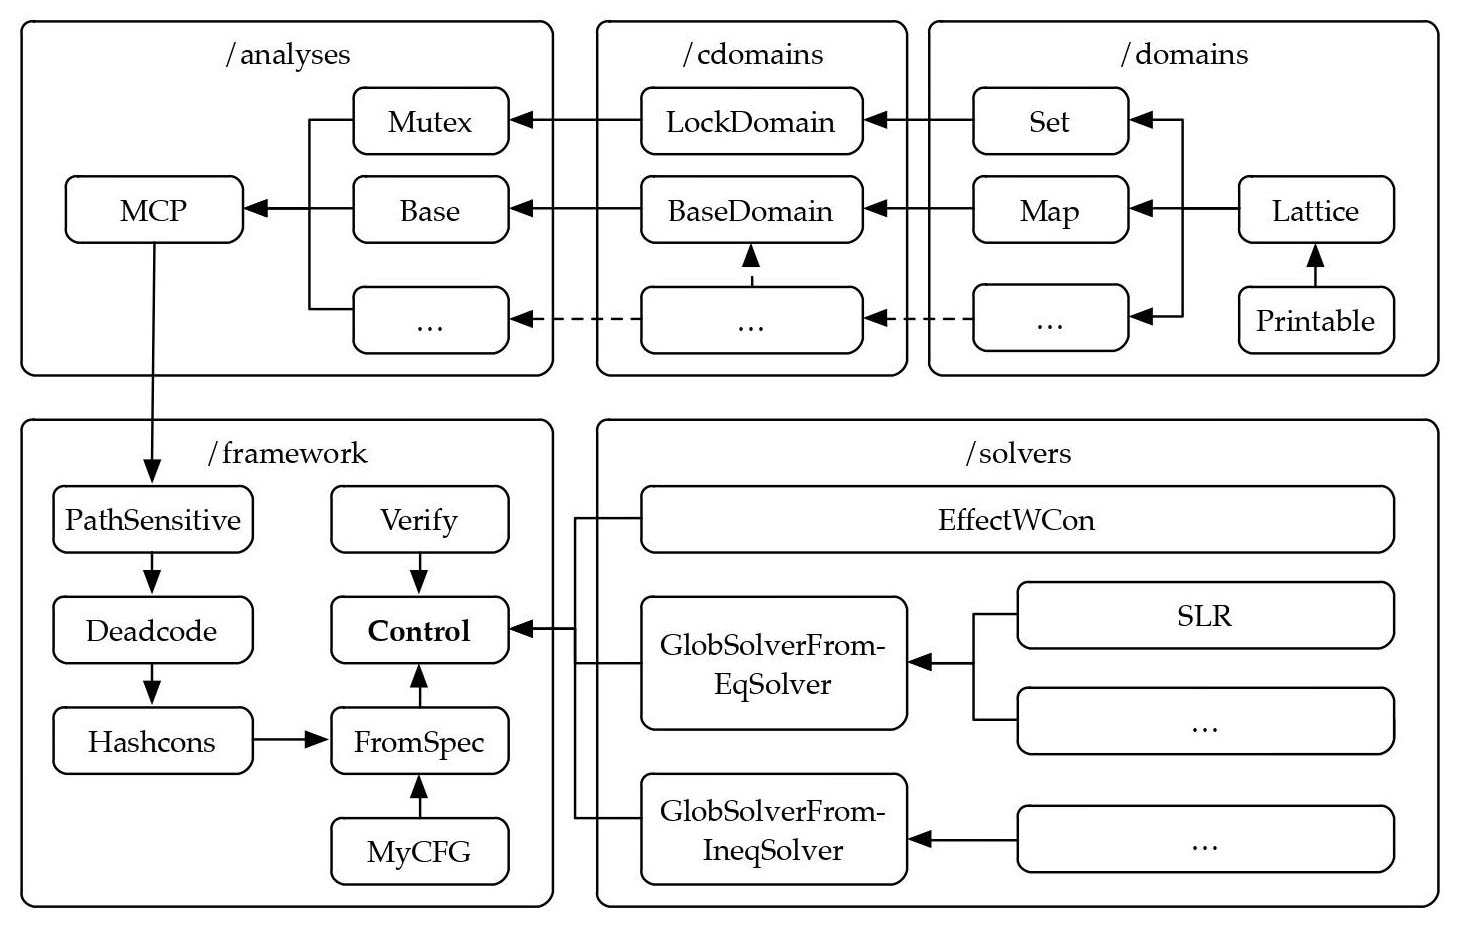
\includegraphics{../figures/goblint_structure_detailed.jpg}
    \caption{Schematic directory structure of \gob. Adapted from \parencite{apinis2014frameworks}}
    \label{fig:gob_structure_detail}
  \end{figure}

    \subsection{Taint analysis}\label{sec:implTaint}
      To define an analysis the \gob\ analyzer provides an interface, where the most relevant parts can be seen in \autoref{fig:analysis_interface}. This interface requires two modules \texttt{D} and \texttt{C} which define the domain and the context-sensitive part of the domain. It also requires the following functions: 
      \begin{itemize}
        \item \texttt{name} to uniquely refer to an analysis.
        \item \texttt{startstate} to define the state used when entering the analysis (similar to $\textsf{init}^{\#}$ from \autoref{chapter:background}).
        \item \texttt{query} to implement the query system of \gob. This allows an analysis to broadcast information to be used in analyses.
        \item \textit{Transfer functions} which define the abstract effects of actions (similar to $[\![A]\!]^{\#}$ from \autoref{chapter:background}).
        \item \textit{Functions for interprocedural analysis}
        \item \textit{Functions for the analysis of multithreaded programs}
      \end{itemize}

      For our taint analysis we create a new module implementing this interface.\\
      As a \texttt{name} for \gob\ internally we chose \texttt{taintPartialContexts} because \texttt{taint} was already used, and the \texttt{name} needs to be unique. In the following we explain in detail how our new analysis module implements the given interface:

      \begin{figure}
        \centering
        \lstinputlisting[language={[Objective]Caml}, breaklines=true, breakatwhitespace=true]{../code/analyses.ml}
        \caption{Simplified Interface for implementing analyses in \gob}
        \label{fig:analysis_interface}
      \end{figure}

      \subsubsection{Domain}
        We need to choose the domain \texttt{D} and the context domain \texttt{C}. According to the concept of our analysis described in \autoref{sec:formalTaint} the domain should be a set of variables. However, we are now analyzing the C language instead of our toy language. In C not every left-hand side of an assignment is just a simple variable, but can be one of many more complex thing, e.g., the memory location \texttt{*xptr} pointed to by the pointer \texttt{xptr}, the fourth place \texttt{a[3]} in an array \texttt{a}, the member \texttt{frac.n} of a struct \texttt{frac} and many more. All these options are described by a concept called \ac{lval}. There is an implementation of this type provided by \gob\ in the \texttt{Lval.CilLval} module. To be as precise as possible we use a set of \ac{lval}s instead of a set of variables for the implementation of the taint analysis.\\
        Another point worth mentioning is that we sometimes need the notion of "all variables" (or rather "all \ac{lval}s") when we want to express that everything is tainted. While conceptually using the full set $X$ poses no issue, in a concrete implementation this is extremely impractical and not even realizable if the set is infinitely large. For this case \gob\ provides a parametrized domain \texttt{ToppedSet(Base)}. This domain is either a set of elements of the \texttt{Base} type or alternatively a \texttt{Top} element which can be interpreted as the "full set of all \texttt{Base} elements". Therefore, we finally have \texttt{D = ToppedSet(Lval.CilLval)} for our domain. Note that this also defines the ordering on the domain to be the regular subset ordering.\\
        It remains to define the module \texttt{C}: We noted in \autoref{sec:formalTaint} that our analysis by itself is context-insensitive. Therefore, the context domain of our analysis \texttt{C} is empty, which is expressed with the \texttt{Unit} domain provided by \gob. Note here, that this does not mean that the taint analysis is always performed context insensitively, i.e., it is only performed once per function. Since \gob\ uses a compound domain, there may be other context-sensitive analyses, forcing the whole compound analysis to analyze a function multiple times. Our taint analysis however never contributes differing sub contexts to the compound context.

      \subsubsection{The \texttt{startstate} function}
        This function computes the initial state for our analysis similar to the $\textsf{init}^{\#}$ function we introduced in \autoref{chapter:background}. As discussed in \autoref{sec:formalTaint}, we implement this function so that it returns the empty set.\\
        We note here however, that in practice we do not use the way, \texttt{startstate} is implemented in the scope of our thesis. In \gob\ this function is called before the main function is even entered. Thus, \texttt{enter} (which we define later) is still used to compute the entry state for the main function. We chose to implement \texttt{startstate} in this way for consistency.

      \subsubsection{Transfer functions}
        These functions implement the effect of actions on the state, similar to the abstract effects of actions $[\![A]\!]^{\#}$ in \autoref{chapter:background}. FOr example \texttt{branch} handles checks for if-statements and loops. For this and most other actions our analysis just propagates the state from before, so they use the default implementation from the \texttt{Analysis.IdentitySpec} of \gob. The default implementations of \texttt{Analysis.IdentitySpec} propagate the given state without change for any action.\\
        Much more interesting is the case of the \texttt{assign} function which handles the effect of an assignment to an \ac{lval}. For this case we want to add the \ac{lval} to our tainted set. The parameters for the \texttt{assign} function are: \texttt{ctx} which amongst other things contains the state from before, the \ac{lval} to which a value is assigned and an expression that evaluates to this value that is assigned. We are only interested in \texttt{ctx} and the \ac{lval}, as for the taint analysis only the fact that a value is assigned is relevant and not its concrete value.\\
        Tainting \ac{lval}s is not as straightforward as it might seem at first. Just adding it to the state from before, i.e., the tainted set, only suffices if the \ac{lval} is a specific location in the memory, e.g., a specific (local or global) variable. The \ac{lval} could however also be a reference to a location in the memory, e.g., a pointer. For these it is not helpful to just taint the reference because we need to know the specific memory locations that are or could be tainted. To solve this issue we make use of \gob's \texttt{MayPointTo} query. This takes a reference to the memory and asks all other activated analyses if they have any information about where this reference may point to. Just like everything else in the static analyzer \gob, the answer is an overapproximation, so we can be sure not to miss any location that could be referenced.\\
        In conclusion, tainting an \ac{lval} goes as follows: If the \ac{lval} is a specific memory location, this \ac{lval} is added to the tainted set. If it is a reference to the memory described by some expression, send a \texttt{MayPointTo} query to ask other analyses which memory locations this expression may point to and add the returned set of \ac{lval}s to the tainted set. We implemented this functionality in a helper function \texttt{taint\_lval}. Therefore, calling this function is the only thing the \texttt{assign} function needs to do as seen in \autoref{fig:assign}.

        \begin{figure}
          \centering
          \lstinputlisting[language={[Objective]Caml}]{../code/assign.ml}
          \caption{Implementation of the helper \texttt{taint\_lval} and the \texttt{assign} function}
          \label{fig:assign}
        \end{figure}

      \subsubsection{Functions for interprocedural analysis}
        Here we define the functions \texttt{context}, \texttt{enter} and \texttt{combine}. These functions work similar to their abstract counterparts as described in \autoref{chapter:background}. In addition to these known functions, the interface also requires two additional functions: \texttt{return} which handles return statements right before a function is left and \texttt{special} which handles calls to library functions or other functions, for which we do not have the source code we can analyze.\\
        Our implementation does not differ a lot from the proposed formal description in \autoref{sec:formalTaint}. Since we are analyzing C and not our toy language, the only major difference is that we need to handle return values and function arguments. Therefore, we implement these functions as follows:

          \paragraph{\texttt{context}:} Our context domain is the \texttt{Unit} domain, and we do not want to generate different contexts for this analysis. Thus, this function always returns the unit element. 

          \paragraph{\texttt{enter}:} Like we discussed in \autoref{sec:formalTaint}, this function always returns the empty set, which is the entry state for the called function.

          \paragraph{\texttt{combine}:} The \texttt{combine} function first checks if there is an \ac{lval} to which the return value is assigned. If so, it taints this respective \ac{lval} in the caller state using the helper function \texttt{taint\_lval} introduced in the "Transfer Functions" section. After that it computes the union of the resulting state with the returned callee state and returns it.\\
          Summarized, the result of this function is the union of both states it receives for combining. It additionally adds \ac{lval}s which are possibly tainted by the return value.

          \paragraph{\texttt{return}:} In our formal description in \autoref{sec:formalTaint}, the $\textsf{combine}^{\#}_\textsf{t}$ function removed variables unreachable by the caller. In the concrete implementation, we give this functionality to the \texttt{return} function, so the removal happens right before the combine. We also remove function arguments as these are unreachable by the caller similar to local variables.
          It is worth pointing out that we do not just remove all \ac{lval}s corresponding to local variables or arguments. A function might exist multiple times in the current call stack, e.g., when the function is recursive. This can result in the existence of multiple versions of the same local variable. \gob\ treats these as being the same variable. Thus, when we remove a local variable we risk also removing a different version of it lower in the call stack, for which we still need the taintedness information. To address this issue, \texttt{return} sends an \texttt{IsMultiple} query for each variable to be removed and only removes those, that surely not have multiple versions. This query is already provided by \gob.

          \paragraph{\texttt{special}:} This function addresses library functions or other functions, for which we do not have the source code to analyze. The simple way to handle these, is to just return Top, i.e., saying "everything could be tainted", after a special call.\\
          This is how we handle unknown functions, however \gob\ provides "Library Descriptors", which contain information about some known C library functions, e.g., \texttt{printf}, \texttt{malloc}, \texttt{cos}, etc. With the respective Library Descriptor of a function, we can gain information about which addresses are "shallowly" written and which are "deeply" written by the call. Shallowly written addresses point to \ac{lval}s which might be directly written. Deeply written addresses however point to \ac{lval}s where not only the \ac{lval} itself, but possibly anything it might recursively point to could be written. Therefore, the \texttt{special} function makes use of \gob's \texttt{MayPointTo} and \texttt{ReachableFrom} queries in the following way:\\
          First the function checks if a Library Descriptor is available. If not, Top is returned. Otherwise, the shallowly and deeply written addresses are obtained from the Descriptor. Consequently, the union of 
          \begin{itemize}
            \item the state before the call
            \item anything that is possibly tainted by the return value (using \texttt{taint\_lval} like in \texttt{combine}) 
            \item the set of \ac{lval}s returned by the \texttt{MayPointTo} query for any shallowly written address
            \item the set of \ac{lval}s returned by the \texttt{ReachableFrom} query for any deeply written address
          \end{itemize}
          is returned by the \texttt{special} function.

      \subsubsection{Functions for the analysis of multithreaded programs}
        To be able to analyze multithreaded programs, \gob's analysis interface requires the following functions: \texttt{threadenter} to compute the startstate for the newly created thread and \texttt{threadspawn} which computes the effect of a thread creating instruction to the state of the creating thread.\\
        We implement the former of these two functions similarly to our \texttt{startstate} and \texttt{enter}. Thus, \texttt{threadenter} returns the empty set.\\
        To implement the other function, \texttt{threadspawn}, we consider how a thread creation effects the state of the creator. We note that for our notion of taintedness the only relevant effect is, that the thread creating function may write thread ID variables to which it receives a reference as an argument. Thus, this function uses the helper function \texttt{taint\_lval} defined in the "Transfer Functions" section to add possibly tainted \ac{lval}s to the state from before and returns the result.

      \subsubsection{The \texttt{query} function}
        We want to enable our taint analysis to tell other analyses which \ac{lval}s are tainted at a specific program point. Therefore, we add a new query \texttt{MayBeTainted} to the query system of \gob. The result of this query should be a set containing \ac{lval}s which may be tainted, i.e., any \ac{lval} that is not in the returned set is definitely untainted.\\
        After this addition we are able to make our \texttt{taintPartialContexts} analysis answer to this query. Therefore, our analysis implements the \texttt{query} function in such a way that it answers only to \texttt{MayBeTainted} queries with the current state but does not answer other queries.

    \subsection{Benefiting other analyses}\label{sec:improveVariableAnalyses}
    In this section we discuss how we improved other existing analyses in \gob\ using the taint analysis we implemented in \autoref{sec:implTaint}.
    \subsubsection{Improving the \texttt{base} analysis}
      The main analysis that benefits from the taint analysis is the \texttt{base} analysis of \gob. This analysis implements a very much extended approach of the basic values-of-variables analysis we formally defined in \autoref{chapter:background}. The \texttt{base} analysis is however still based on the main goal and basic concept of finding a mapping from program variables to possible values at each program point. Therefore, this analysis uses a mapping from variables to their possible values as part of its domain. However, here the \texttt{ValueDomain} of the mapping is much more complex than just a set of possible integers. It provides abstractions for virtually any type in C, including arrays, structs and pointers. Even more though, the \texttt{ValueDomain} is highly configurable. Amongst other options it allows choosing between different ways of abstracting integer values or arrays. One interesting option related to the topic of this thesis is the possibility to choose between different degrees of context sensitivity: the analysis can be fully context-sensitive, insensitive with respect to integer variables (abstracted by intervals or in general), only sensitive with respect to pointers or completely insensitive. When choosing anything but the completely context-sensitive option, this analysis experiences the (avoidable) loss of precision described in \autoref{sec:precisionLoss}.\\
      To reduce this loss we need to change the \texttt{combine} function of the \texttt{base} analysis so that it uses the results of our \texttt{taintPartialContexts} analysis. In order to get a better understanding of what needs to be changed, we first describe how the \texttt{combine} function was implemented before our changes:
      \begin{enumerate}
        \item The return value is saved. Its value is removed from the callee state.
        \item All globals are removed from the caller state.
        \item Everything from the callee state is added to the caller, possibly overwriting caller values. This excludes the return value which is handled separately.
        \item Some further adjustments according to the configuration are performed to the resulting state.
        \item The saved return value is added to the state before it is returned.
      \end{enumerate}
      To implement our changes we will focus on the steps 2 and 3, where the caller mapping is updated. The other steps will remain the same.\\
      The core idea to implement the concept proposed in \autoref{sec:formalImprove} is as follows: First we get the set of possibly tainted \ac{lval}s from the callee. We then iterate over its elements one by one, where for each tainted \ac{lval} we update the caller mapping with the corresponding value from the callee mapping, i.e., we get the value corresponding to that \ac{lval} from the callee mapping and set the \ac{lval} to map to this value in the caller mapping. This functionality of updating the caller mapping with the callee mapping using the tainted set is implemented in a helper function \texttt{combine\_st}.\\
      Before we explain how this helper function is implemented, we first show how it is embedded in the current implementation of the \texttt{combine} function. As discussed, we alter steps 2 and 3: First we send a \texttt{MayPointTo} query to the return state of the callee. We then check if the query returned the Top set, i.e., the notion that everything is tainted. In this case we perform the unchanged steps 2 and 3 just like before. Amongst other cases, this can happen, when the \texttt{base} analysis is run without our taint analysis being activated.\\
      We now define what happens, when the result of the query is an explicit set. Before calling the helper function \texttt{combine\_st}, we have to handle two special cases here:
      \begin{itemize}
        \item For a global variable, there is no mapping in the callee state, but there is one in the caller state. This case can occur in multithreaded mode, if this variable was protected by a mutex before the call, but the mutex was released in the called function. In this case, the mapping for this variable would be removed from the state within the callee. In the \texttt{combine} function, we do need to keep this new information from the callee for such a variable, i.e., remove it from the caller mapping. Therefore, we filter over the caller mapping and remove all globals, for which there exists no mapping in the callee mapping.

        \item For a global variable, there is a mapping in the callee state, but there is none in the caller state. This case can occur if new information is gained within the call, e.g., some new memory is allocated. This information is not tracked by the tainted set and would therefore not be copied into the caller state. Since we still want to have this new information after the combine, we add all these mappings from the callee to the caller.
      \end{itemize}
      These cases have to be handled separately, as for these the corresponding \ac{lval} is not necessarily contained in the tainted set. After the two special cases are handled, we use the \texttt{combine\_st} helper function to finally update the tainted \ac{lval}s in the caller state. We then proceed with the resulting state to the steps 4 and 5 like before.\\
      We note here that we added a new parameter \texttt{f\_ask} to the \texttt{combine} function. To do this we had to update the analysis interface and consequently all analyses implementing it. This new parameter allows the analyses to send queries to the returned callee state, which was not possible before.
      \paragraph{\texttt{combine\_st}:} This helper function takes the caller state (updated according to the two special cases), the callee state and the set of tainted \ac{lval}s. The difficulty here is, that while the tainted set is a set of \ac{lval}s, the mappings from the states of the \texttt{base} analysis are mappings from variables to abstractions of their possible values. This means, that our tainted set may include specific places in an array or specific members of a struct, e.g., \texttt{a[3]} and \texttt{frac.n}. In contrast to this, the mappings we want to combine do not map \texttt{a[3]} and \texttt{frac.n} to abstract values, but rather map \texttt{a} to some abstraction of an array and \texttt{frac} to some abstraction of a struct. To solve this issue we make use of the \texttt{get} and \texttt{set\_savetop} functions provided by the module of the \texttt{base} analysis. With these functions it is possible to get and set values of addresses to specific \ac{lval}s in a variable mapping of the \texttt{base} analysis.\\
      Therefore, the implementation of this function goes as follows: We fold over the tainted set. For each \ac{lval} we build an address to this \ac{lval}. Then we try to \texttt{get} the value this address points to from the callee state. If this returns a value, we use \texttt{set\_savetop} to update the caller state, i.e., set the address to the value we got. Otherwise, we proceed with the next \ac{lval}.\\
      There are however a few special cases to handle: One issue is that in \gob\ there exists a domain for abstracting array values called "partitioned array". This abstraction saves an index which it uses to split an array into three parts: The group of all values to the left of the index, the value at the index itself and the group of all values to the right. Each of the three parts is abstracted with a collective value. The index can be either a specific integer or a variable.\\
      For array variables abstracted with this "partitioned array" domain, copying \ac{lval}s one by one does not work, as the information of the partitioning is lost when we attempt it. Therefore, we check if the current value corresponds to a place in an array abstracted with the "partitioned array" domain and if so, we copy the whole partitioned array from the callee mapping to the caller mapping.\\
      A similar issue occurs with values of void type, as for these the \texttt{get} does not work correctly. Therefore, we get the value for the corresponding variable from the callee mapping itself and update the caller mapping with it.\\
      The last issue we need to address is again related to partitioned arrays. Recall, that an array can be partitioned by the value of a variable. This means, that if a variable is tainted which is used as a partitioning index, the partitioned array in the caller mapping is invalid. Therefore, for each \ac{lval} we check if it corresponds to a variable partitioning an array. If so, we update the caller state by copying all abstracted arrays which are partitioned by the variable in question from the callee mapping to the caller mapping. This is possible, because the state of the \texttt{base} analysis keeps track of which arrays are partitioned by certain variables.\\
      Finally, after we are done folding over all tainted \ac{lval}s, the function returns the modified caller state.
      %TODO: Summarize the updated combine

    \subsubsection{Improving other Variable Analyses}
      In \gob\ there are multiple other analyses which can be described by our notion of a variable analysis. For some of these we are able to the precision loss of partial contexts by using the results from our \texttt{taintPartialContexts} analysis. We briefly discuss the details of these improvements in this section:

      \paragraph{The \texttt{varEq} analysis:}\mbox{}\\
        This analysis tracks, which \ac{lval}s definitely hold the same value, irregardless of what this value is. As an example, after an assignment \texttt{a[3] = y;} this analysis propagates the information that \texttt{a[3]} and \texttt{y} in an equality set, until either \texttt{a[3]} or \texttt{b} are written.\\
        One can construct a case, where a function \texttt{f()} is called twice, once where some equality \texttt{x = y} holds and once where it does not hold. We assume that \texttt{x} and \texttt{y} are not altered within \texttt{f()}. If the \texttt{varEq} analysis is performed context insensitively, we would lose the equality information when the \texttt{combine} is performed after both calls. This is because the equality information is discarded when the entry states are joined.\\
        So far, the \texttt{combine} function just propagated the callee return state. This can be improved in the following way: We obtain the tainted set and remove all equality sets containing at least one tainted \ac{lval} from the caller state. Then we compute the greatest lower bound of the resulting caller state and the callee state. This means, we compute a state that unifies the information from the caller state without tainted \ac{lval}s with the information from the callee state.\\
        In the example from above this changed \texttt{combine} allows the analysis to keep the equality \texttt{x=y} when the taint analysis is activated.

      \paragraph{The \texttt{relation} analysis:}\mbox{}\\
        This analysis tracks relations between variables. The analysis can be configured to use different kinds of relations implemented in different domains. An example for these domains is the octagon domain, which works with relations of the form $\langle x \rangle + \langle y \rangle \geq 0$, where $\langle x \rangle$ stands for either $x$ or $-x$. The relation analysis is parametrized in such a way that our changes apply to the analysis independent of the selected relation domain.\\
        The case where this analysis unnecessarily loses precision because of context insensitivity, is similar to the one discussed in the paragraph discussing the improvement of the \texttt{varEq} analysis: A function \texttt{f()} is called twice, where some relation between the variables \texttt{x} and \texttt{y} once holds and once does not hold. When the entry states for both calls are joined, the relation in question is removed and is therefore missing after the call. We once again assume that \texttt{x} and \texttt{y} are not altered within \texttt{f()}.\\
        Before we apply our changes, the \texttt{combine} function of the \texttt{relation} analysis is implemented so that it removes all information related to global variables from the caller state and merges the result with the callee state. The result contains the relations from the caller that are not related to globals and all relations from the callee.\\
        Accessing the result of our taint analysis via a query, we can improve this way of combining. We achieve this by only removing relations related to tainted global variables and keep those that only relate to locals and untainted globals. After that, the result is merged with the callee state like before.\\
        We note here, that this analysis tracks relations between variables while our tainted set contains tainted \ac{lval}s. Therefore, we convert the set of tainted \ac{lval}s to a set of tainted variables. This is easily possible, since all \ac{lval}s in our tainted set refer to variables or specific parts of variables. In particular, they do not point to some memory location, which would make identifying a corresponding variable difficult.

      \paragraph{The \texttt{condVars} analysis:}\mbox{}\\
        This analysis tracks equalities between variables and logical expressions. Take the following statement as an example: \texttt{tv = (c == 0);}. For this statement, the \texttt{condVars} analysis tracks, that the variable \texttt{tv} holds the value of the logical expression \texttt{c == 0}. This information can be used, when there is an \texttt{if} statement, checking whether \texttt{tv} is true or not. Knowing \texttt{tv} is equal to \texttt{c == 0}, this analysis can provide the information that \texttt{c == 0} evaluates to \texttt{true} in the \texttt{true}-branch of the \texttt{if} statement.\\
        Currently, the \texttt{combine} function of this analysis is implemented to discard the callee return state and remove all information related to global variables from the caller state. This results in the loss of all information related to globals whenever a function is called, irregardless whether the \texttt{condVars} analysis is performer context sensitively or insensitively.\\
        We can improve this by only removing information related to tainted globals from the caller state and keeping information related to untainted globals. This makes the \texttt{condVars} analysis more precise whenever the \texttt{taintPartialContexts} analysis is activated. Again we note here, that this analysis is concerned with information related to variables, not \ac{lval}s. Therefore, we convert the set of tainted \ac{lval}s to a set of tainted variables like in the previous paragraph. 
      
% !TeX root = ../main.tex
% Add the above to each chapter to make compiling the PDF easier in some editors.

\chapter{Combatting the Precision Loss of Thread Analyses}\label{chapter:precisionLossThreadAnalyses}
% local traces
  To (((Something))) M. Schwarz et al. \parencite{schwarz2023clustered}.
  \section{Theory}\label{sec:threadTheory}
  In Chapter 6 of their paper \parencite{schwarz2023clustered} they propose an analysis that identifies threads by their creation history. Among other things, this analysis helps to identify which threads are unique and which actions may or may not happen in parallel.\\
  As mentioned, threads are identified by their creation history, which is used as an ID to identify different threads. This history is a sequence of create edges starting with $\textsf{main}$. To prevent such a history to grow to infinity, they define the notion of non-unique thread IDs which may identify multiple threads each.\\
  Formally, the set of possible abstract thread IDs $\mathcal{I}^{\#}$ is $(\textsf{main}\cdot\mathcal{P}^*) \times 2^{\mathcal{P}}$, where $\mathcal{P}$ is the set of create edges and $\mathcal{P}^*$ a sequence of such edges. $\langle u, f \rangle \in \mathcal{P}$ refers to an outgoing edge from program point $u$ which creates a thread starting at $f$.
  In this notion, IDs of the form $(i, \emptyset) \in \mathcal{I}^{\#}$ are unique, while $(i, s) \in \mathcal{I}^{\#}$ are not unique if $s \neq \emptyset$.\\
  \\
  As mentioned, these abstract thread IDs are found by a dedicated thread ID analysis. In order to work correctly, this analysis needs to track the current thread ID as well as a set of create edges already encountered. Thus, the abstract domain for this analysis is $\mathbb{D}_\textsf{tID} = (\mathcal{I}^{\#} \times 2^{\mathcal{P}})$. An element $(id, es)$ of this domain is the product of the current thread ID $id$ and the set of encountered create edges $es$.\\
  The main part of the analysis now works as follows: Assume a thread-create edge $(u, create(f), v)$ is encountered with a state $(id, es)$. When the $id$ is already non-unique, the new thread is identified with a (possibly new) non-unique ID. In the other case $id$ is unique, i.e., $id = (i, \emptyset)$. Then the analysis checks whether the currently encountered edge was already encountered before, i.e., if it is present in the set of encountered edges $es$. If not, the new thread is identified with a new unique ID that is created by appending the current create edge to the first part of $id = (i, \emptyset)$. Otherwise, the new thread is identified with a non-unique ID.\\
  % TODO: Formally?
  It is worth mentioning, that the $\textsf{combine}^{\#}_\textsf{tID}$ function is implemented to ignore the caller state and propagate the callee return state for this analysis.
  \\
  As of now the thread ID analysis is always run context sensitively, i.e., $\mathbb{C}_\textsf{tID} = \mathbb{D}_\textsf{tID}$ and $\textsf{context}^{\#}_\textsf{tID}\ D = \textsf{enter}^{\#}_\textsf{tID}\ D$. Performing it context insensitively is not practical. The reason for that is leads to cases where a least upper bound of two states $(id_1, es_1)$ and $(id_2, es_2)$ has to be computed. Since abstract IDs from $\mathcal{I}^{\#}$ are not reasonably comparable, this leads to a notion of "unknown thread ID" or "any possible thread ID" which we want to avoid.\\
  It is much more reasonable to run the thread ID analysis partially context sensitively, where contexts are differentiated with respect to the current $id$ but not the set of encountered create edges $es$. Computing the least upper bound of sets of encountered create edges is reasonably possible by taking the union of the sets. With these insights we can perform the thread ID analysis partially context sensitively with
  \[\mathbb{C}_\textsf{tID} = \mathcal{I}^{\#} \text{ and } \textsf{context}^{\#}_\textsf{tID}\ (id, es) = id\]
  When we now run this partially context-sensitive analysis, it is possible to encounter cases where precision is lost similarly to how we described it in \autoref{sec:precisionLoss}. We show this with the example program from \autoref{fig:example_thread}. In this program, \texttt{procedure()} is called two times, once without a thread being created beforehand and once with a thread created. For now this thread created in \autoref{code:create} has the unique ID $([main \cdot \langle u_2, s_{tproc} \rangle])$, assuming the program point before the \texttt{create(tproc)} is $u_2$ and $s_{tproc}$ is the start point of the thread procedure \texttt{tproc()}. The two entry states for \texttt{procedure()} are $(([main], \emptyset), \emptyset)$ and $(([main], \emptyset), \{\langle u_2, s_{tproc} \rangle\})$, as once the edge $\langle u_2, s_{tproc} \rangle$ was encountered and once it was not. These states both have the same context, i.e., $([main], \emptyset)$, and thus their entry states are joined. The result is the same as the second entry state $(([main], \emptyset), \{\langle u_2, s_{tproc} \rangle\})$. Since we assume for this example, that no thread was created in \texttt{procedure()}, the return state is the same as the joined entry state. With the way, the $\textsf{combine}^{\#}_\textsf{tID}$ function is defined, this state is used for the point after both calls. In particular, it is used for the state after the call in \autoref{code:proc1}. Thus, the \texttt{create()} action in \autoref{code:create} is actually encountered again with the state $(([main], \emptyset), \{\langle u_2, s_{tproc} \rangle\})$. The result of this is, that the thread created here is now identified with a non-unique abstract ID $([main], \{\langle u_2, s_{tproc} \rangle\})$, because this create edge is in the set of encountered create edges.\\
  With this result, some possible race condition are detected, even though in fact there are none in this program. For once, The thread created in \autoref{code:create} is no longer identified with a unique edge. Thus, it is no longer possible to know that only one thread runs with the procedure \texttt{tproc()} and consequentially, only one thread can perform the assignment instructions in \autoref{code:assign2}. Therefore, a data race is found for this assignment.\\
  Furthermore, it is no longer possible to identify, that no thread has been crated before the variable assignment in \autoref{code:assign1}, because $\langle u_2, s_{tproc} \rangle$ is in the set of encountered create edges of the state at this point. Thus, a possible data race is found also for this assignment instruction.\\
  It is worth mentioning here, that the process we described above is adapted to be better understandable for the reader. Following the actual definitions of static analysis, the corresponding system of constraints for the program points is generated. For this system a solution can be computed with a fix-point solver.\\

  \begin{figure}
    \centering
    \begin{subfigure}{.35\textwidth}
      \centering
      \lstinputlisting[escapechar=|, language=C]{../code/04-example_thread.c}
    \end{subfigure}
    \caption{Example program to illustrate the precision loss of partial contexts in the thread ID analysis}
    \label{fig:example_thread}
  \end{figure}
  To combat this loss of precision, we propose a "thread-create" analysis. This analysis checks for each procedure, whether a thread is possibly created between the entry to it and the return. Note that it does not matter, if a thread is created in the procedure itself or in another procedure which the procedure called. The domain we use for this analysis is the set of boolean values $\mathbb{D}_\textsf{tc} = \{\textsf{true}, \textsf{false}\}$. The analysis tracks whether a procedure \textit{may} create a thread. Thus, we encode uncertainty, i.e., "a thread \textit{may} have been created" with $\textsf{true}$. Similar to the taint analysis from \autoref{sec:formalTaint}, this analysis is context insensitive by itself and thus, $\mathbb{C}_\textsf{tc} = \{\bullet\}$.\\
  In conclusion, the state at some program point $\eta_\textsf{tc}\ [v,\bullet]$ answers the question "\textit{May} a thread have been created since the entry of the current procedure up to the node $v$?".\\
  In the following we give the definitions of the analysis functions for this function:
  \begin{align*}
    \textsf{init}^{\#}_\textsf{tc} &= \textsf{false}\\
    [\![ A ]\!]^{\#}_\textsf{tc}\ c &= \left\{ \begin{array}{ll}
      \textsf{true} & \text{if }A \equiv (create(f);)\\
      c & \text{else}
    \end{array} \right. \\
    \textsf{enter}^{\#}_\textsf{tc}\ c &= \textsf{false}\\
    \textsf{combine}^{\#}_\textsf{tc}\ (c_\textsf{cr}, c_\textsf{ce}) &= c_\textsf{cr} \lor c_\textsf{ce}\\
    \textsf{context}^{\#}_\textsf{tc}\ c &= \bullet\\
  \end{align*}
  
  We note that $\textsf{init}^{\#}_\textsf{tc}$ and $\textsf{enter}^{\#}_\textsf{tc}$ return $\textsf{false}$, because at the beginning and whenever a procedure is entered, no thread has been created yet in the current procedure. After a call, the state should be $\textsf{true}$ if a thread was created by the caller before or if one was created by the callee. Thus, the $\textsf{combine}^{\#}_\textsf{tc}$ function returns the result of a locical "or" operation on both states.\\
  \\
  With this analysis, we can improve the $\textsf{combine}^{\#}_\textsf{tID}$ of the thread ID analysis. Before, this function was defined as $\textsf{combine}^{\#}_\textsf{tID}\ (D_\textsf{cr}, D_\textsf{ce}) = D_\textsf{ce}$. We change this, so this analysis only returns the callee state when a thread was possibly created in the call and otherwise returns the caller state from before:
  \[\textsf{combine}^{\#}_\textsf{tID}\ (D_\textsf{cr}, D_\textsf{ce}) = \left\{ \begin{array}{ll}
    D_\textsf{ce} & \text{if } \eta_\textsf{tc}\ [e_f,c]\\
    D_\textsf{cr} & \text{else}
  \end{array} \right.\]
  for an edge $(u, f();, v)$ where $c$ is the corresponding context.\\
  This modification allows the analysis to keep the callee state with the respective set of encountered edges. In the example from \autoref{fig:example_thread} this means, that after the call in \autoref{code:proc1}, the state from before with no encountered edges is kept. This results in no race being detected in \autoref{code:assign1}. Furthermore, because the thread created in \autoref{code:create} is known to be unique, no race is detected in \autoref{code:assign2}.

  \section{Implementation}
    We briefly described in this section, how we implemented the thread-create analysis from the previous chapter in \gob\ and how we used it to improve the \texttt{threadId} analysis that already exists in the analyzer.\\
    Similar to the \texttt{taintPartialContexts} analysis from \autoref{sec:implTaint}, we implement a new module \texttt{threadCreate} that implements the interface seen in \autoref{fig:analysis_interface}. In the following we just discuss the implementation of the functions and modules required by the interface. Their meaning to the analyzer is explained in \autoref{sec:implTaint}.

    \paragraph{Domain:}\mbox{}\\
    The Domain \texttt{D} for this analysis only contains the two boolean values, where \texttt{false} stands for "definitely no thread was created" and \texttt{true} for "maybe a thread was created". For this \gob\ provides the \texttt{MayBool} domain implementing this notion with the corresponing ordering.\\
    Similar to the taint analysis, this analysis does not contribute to the overall context of the analyzer, and thus we chose \texttt{Unit} for the module \texttt{C}.

    \paragraph{The \texttt{startstate} function:}\mbox{}\\
    The analysis starts with the state that no thread was created and thus \texttt{startstate} returns \texttt{false}.

    \paragraph{Transfer functions:}\mbox{}\\
    Only actions that create a thread have an effect on the state of this analysis. Hence, all regular transfer functions propagate the state from before without any changes.

    \paragraph{Functions for interprocedural analysis:}\mbox{}\\
    For this analysis these functions are implemented as follows:
    \begin{itemize}
      \item \texttt{context}: With the context domain being \texttt{Unit} this function returns the unit element
      \item \texttt{enter}: When entering a function we want to start with a state describing, that no thread was created by this function yet. Thus, the \texttt{enter} function returns \texttt{false}
      \item \texttt{combine}: After returning from a function call, the state should be \texttt{true} if a thread was created by the caller before or by the callee. Therefore, the \texttt{combine} function joins the caller state and the callee return state with a logical \texttt{or}. 
      \item \texttt{return}: This function propagates the state from before.
      \item \texttt{special}: If the special function that is called here is a thread creating function, e.g., \texttt{pthread\_create()}, the state afterwards is \texttt{true}, since a thread has just been created. If the function is unknown, \texttt{true} is returned as well, because a thread might have been created. In all other cases, the previous state is propagated. 
    \end{itemize}

    \paragraph{Functions for the analysis of multithreaded programs:}\mbox{}\\
    We implement the \texttt{threadspawn} function similar to the \texttt{startstate} function. When a thread is entered, the starting state for this thread is \texttt{false}, i.e., no thread has been created yet.\\
    The \texttt{threadCreate} function returns \texttt{true}, because it created a thread and that is what the state is tracking.

    \paragraph{The \texttt{query} function:}\mbox{}\\
    To allow the new thread-create analysis to broadcast its information to other analyses we add a \texttt{MayThreadCreate} query. This query is answered by the thread-create analysis with the current state. Other analysis can send a \texttt{MayThreadCreate} query to gain the information, whether a thread has been created from the beginning of the current function up to the point where the query is sent. In the case, that the \texttt{threadCreate} analysis is not performed, this query is answered with \texttt{true} by default, i.e., "A thread \textit{may} have been created".\\
    \\
    \\
    \paragraph{Improving the \texttt{threadId} analysis}
    In \gob\ there exists an implementation of the thread ID analysis we introduced in \autoref{sec:threadTheory}, namely the \texttt{threadId} analysis. This analysis was always performed context-sensitively. Thus, we add the option \texttt{ana.thread.context.createEdges} to the analyzer. This option is enabled by default, but it allows for removing the set of encountered create edges from the context when it is disabled. We implement this by changing the \texttt{context} function of the \texttt{threadId} analysis, so that it checks this option.\\
    To implement our proposed improvements, we change the \texttt{combine} function of the \texttt{threadId} analysis according to our proposal from \autoref{sec:threadTheory}. It now sends a \texttt{MayThreadCreate} and returns the caller state when the answer is \texttt{false}. Otherwise, the callee state is returned like before our changes.


% !TeX root = ../main.tex
% Add the above to each chapter to make compiling the PDF easier in some editors.

\chapter{Evaluation}\label{chapter:evaluation}
  In this chapter, we evaluate our approach. This is split into two parts: First, we test, whether our implementation is sound, i.e., it does not lead to wrong results. After that, we benchmark the implementation on some real-world C programs. The goal of the benchmark is to get a perspective on the precision and computation time of our proposed improvements from \autoref{chapter:precisionLossVariableAnalyses} and \autoref{chapter:precisionLossThreadAnalyses}. Thus, we compare context-insensitive runs with our improvement to context-insensitive ones without the improvement and to context-sensitive runs. In particular, we want to know how much of the precision lost by context-insensitivity can be recovered through our proposed improvements.

  \section{Testing}
    This section aims to ensure, that the addition of the \texttt{taintPartialContexts} analysis to \gob\ as described in \autoref{sec:implementation} does not lead to wrong results. Additionally, we want to make sure that just activating the taint analysis on a fully context-sensitive analysis run does not lead to less precise results.\\
    \\
    \gob\ provides an extensive set of regression test cases already. These test edge cases of various features of the analyzer. Each test case comes with a specific configuration, that should be used when executing the test.\\
    To verify our implementation, we ran all regression test cases with their specified configuration but additionally activated the taint analysis. This helps to ensure that no precision is lost, just by activating the taint analysis. These test runs helped to find some bugs, which then were fixed.\\
    For the \texttt{threadCreate} analysis we used the same approach, where we ran all regression tests with the thread-create analysis additionally activated.\\
    We also contributed a few new regression tests which specifically test edge cases of the taint and the thread-create analysis. These include tests for each existing analysis, where we included either of our two new analyses, as well as tests for bugs we cleared to show the correct behavior after the fix. The new regression tests also aim to demonstrate how our changes improve the precision of existing analyses.\\
    \\
    Additionally, we investigate the results of the benchmarks we describe in the following section. These reinforce the verdict that the taint analysis and the thread-create analysis are sound in their implementation.
  
  \section{Benchmarking the improved \texttt{base} analysis}
    In this section, we investigate, if and to what extent the changes we proposed in \autoref{sec:improveVariableAnalyses} provide an improvement. In particular, we compare analyses with different configurations in terms of precision and computation time. However, we focus on benchmarking the changes to the \texttt{base} analysis as this is the main variable analysis used in \gob. We do perform benchmarks with the other variable analyses we improved in \autoref{sec:improveVariableAnalyses} besides the \texttt{base} analysis.
    \subsection{SV-Benchmarks}\label{sec:benchSVbench}
      The first benchmarking approach we will describe in this section uses the SV-Benchmarks' "Collection of Verification Tasks" \parencite{svBench}. This collection of verification tasks is "constructed and maintained as a common benchmark for evaluating the effectiveness and efficiency of state-of-the-art verification technology" \parencite{svBench}. Each verification task consists of a program and a corresponding specification, i.e., a set of properties. The verifier to be benchmarked, i.e., in our case the \gob\ analyzer with our changes, then performs an analysis run on a given program. After that, it is checked, whether the verifier was able to prove the given set of properties. The properties we focus on for our benchmarks are the following:
      \begin{itemize}
        \item \texttt{unreach-call}: A specified function \texttt{reach\_error()} in the program is never called during runtime.
        \item \texttt{no-overflow}: No integer overflow occurs in the program.
        \item \texttt{no-data-race}: The program contains no race condition.
      \end{itemize}
      For each of these properties, we perform three benchmark runs with different configurations on each program for which it is specified that the property holds.
      The three configurations we use for the benchmark runs are:
      \begin{itemize}
        \item \textit{sens}: The \texttt{base} analysis is performed context-sensitively.
        \item \textit{insens}: The \texttt{base} analysis is performed context-insensitively.
        \item \textit{insens taint}: The \texttt{base} analysis is performed context-insensitively with the improvements of the taint analysis.
      \end{itemize}
      During each benchmark run with a certain configuration we save different kinds of information to compare later. The most important of these are the computation time per program and the total number of programs, for which the property to prove was proven.\\
      We first investigate the precision. For this, we compare the number of programs for which the property was proven per configuration and property: The raw numbers can be found in \autoref{fig:resultSVbenchTable}, while the graph in \autoref{fig:resultSVbench} shows a visualization of the results.\\
 
      \begin{figure}[!ht]
        \centering
        \begin{tikzpicture}
          \begin{axis}[
              width=0.7\linewidth,
              ybar=0pt,
              ymin=0,ymax=100,
              xtick=data,
              symbolic x coords={\texttt{unreach-call}, \texttt{no-overflow}, \texttt{no-data-race}},
              enlarge x limits={abs=50pt},
              bar width = 15pt,
              ylabel= \% property proven, 
              ytick align=outside, 
              ytick pos=left,
              major x tick style = transparent,
              %x tick label style={rotate=45},
              legend style={at={(0.04,0.96)},anchor=north east, font=\footnotesize, legend cell align=left,},
              ]    
              \addplot[ybar,fill=TUMAccentGreen, area legend] coordinates {
                (\texttt{unreach-call},18.92263836)
                (\texttt{no-overflow},40.78357328)
                (\texttt{no-data-race},74.30786268)}; 
              \addplot[ybar,fill=TUMAccentOrange, area legend] coordinates {
                (\texttt{unreach-call},18.81450899)
                (\texttt{no-overflow},40.51215483)
                (\texttt{no-data-race},74.41860465)}; 
              \addplot[ybar,fill=TUMBlue, area legend] coordinates {
                  (\texttt{unreach-call},18.61791015)
                  (\texttt{no-overflow},40.59476044)
                  (\texttt{no-data-race},74.41860465)};
          \legend{sens, insens taint, insens}  
          \end{axis}
        \end{tikzpicture}
        \caption{Bar graph for the comparison of the three configurations per property. A bar represents the percentage of programs, for which the corresponding property was proven using the corresponding configuration}
        \label{fig:resultSVbench}
      \end{figure}

      \begin{figure}
        \centering
        \begin{tabular}{l|l||r|r||r|r|r}
          \textit{property} & \textit{config.} & \textit{\# proven} & \textit{\# total} & \textit{\# loss by} & \textit{\# recovered} & \textit{\% recovered}\\
            &  & \textit{tasks} & \textit{tasks} & \textit{insens} & & \textit{of loss}\\
          \hline
          \texttt{unreach-call} & \textit{sens} & 1925 & 10173 & 31 & 20 & 64.52\\
          & \textit{insens taint} & 1914 & & & & \\
          & \textit{insens} & 1894 & & & & \\
          \hline
          \texttt{no-overflow} & \textit{sens} & 3456 & 8474 & 16 & -7 & -43.75\\
          & \textit{insens taint} & 3433 & & & & \\
          & \textit{insens} & 3440 & & & & \\
          \hline
          \texttt{no-data-race} & \textit{sens} & 671 & 903 & -1 & 0 & 0.00\\
          & \textit{insens taint} & 672 & & & & \\
          & \textit{insens} & 672 & & & & \\
          \hline
        \end{tabular}
        \caption{Table showing the results of the SV-Benchmarks.}
        \label{fig:resultSVbenchTable}
      \end{figure}

      As we can see in \autoref{fig:resultSVbench}, there is in fact not a large difference between the three configurations for each property. Our interpretation of this result is, that the choice between our three configurations only has a small effect on the precision of \gob when analyzing real-world programs. In other words, this means, that not a lot of precision is lost by performing the \texttt{base} analysis context-insensitively. The taint analysis can only recover lost precision, so little overall precision loss means, that the taint analysis can only provide little overall improvement.\\
      \\
      We now take a closer look at \autoref{fig:resultSVbenchTable}. We first investigate the results for the \texttt{unreach-call} property: We see, that with the \textit{insens} configuration, the analyzer was able to prove the property 31 times fewer than with the \textit{sens} configuration, which is less than 0.4\% of the total number of tasks. However, it proved the property 20 times more often with the \textit{insens taint} configuration compared to the \textit{insens} configuration. This leads us to the conclusion, that for this property the taint analysis helped to recover about 65\% of the precision lost.\\
      As for the results of the \texttt{no-overflow} property, it seems like the usage of the taint analysis leads to less precise results. This property was proven for 7 fewer programs when using the \textit{insens taint} configuration instead of the \textit{insens} configuration. In fact, these results helped us find a bug in our implementation. This bug is now removed and after the fix, the \texttt{no-overflow} property is proven for these 7 programs with the \textit{insens taint} configuration. In conclusion, however, we cannot say that the taint analysis provides an improvement for proving the \texttt{no-overflow} property.\\
      Similarly, the \textit{insens taint} configuration is exactly as precise as the \texttt{insens} configuration for the \texttt{no-data-race} property. A timeout is the reason, why the \textit{sens} configuration proved the property for one fewer program than both of the other configurations. Considering this, we conclude, that for this property all three configurations are equally precise.\\
      \\
      The table in \autoref{fig:timingSVbenchTable} gives information related to the computation times of this benchmark. We first investigate the average computation time of only the tasks, where none of the runs with different configurations terminated with an error. Errors that occurred are mainly timeouts or stack overflow exceptions. A timeout was set to interrupt a task after fifteen minutes of non-termination. We can see, that the differences in the average computation time of tasks without errors are very small. In the case of the \texttt{unreach-call} property, the \textit{insens taint} configuration actually performed worse than the \textit{sens} configuration on average, but not by much. This is the property, where the taint analysis provided the most improvement as we found in the previous paragraph.\\
      The most interesting property in this comparison is probably \textit{no-overflow}. Here, both the \textit{insens} and the \textit{insens taint} configuration have a significantly lower average computation time than the \textit{sens} property, when taking all tasks into account. The reason for this is, that the number of errors for each of these two configurations is just about a third when compared to the \textit{sens} configuration. From this, we deduce, that performing the \texttt{base} analysis context-insensitively leads to fewer errors and produces results more quickly compared to performing it context-sensitively. As we found in the previous paragraph, not a lot of precision is lost with the \textit{insens} configuration compared to the \textit{sens} configuration. However, the taint analysis did not provide much improvement for this property.\\
      A similar observation can be made from the timing results of the \texttt{no-data-race} condition.  For this property, the observation is far less expressive, as only one timeout occurred for the \textit{sens} configuration, compared to no error for the other configurations.
    
      \begin{figure}
        \begin{tabular}{l|l||r|r||r|r}
          \textit{property} & \textit{config.} & \textit{avg. cputime} & \textit{avg. cputime} & \textit{\# Timeouts} & \textit{\# Errors} \\
          & & \textit{all tasks (s)} & \textit{no errors (s)} & & \\
          \hline
          \texttt{unreach-call} & \textit{sens} & 191 & 30.8 & 1712 & 1934 \\
          & \textit{insens taint} & 188 & 31.2 & 1658 & 1908 \\
          & \textit{insens} & 188 & 28.1 & 1563 & 1799 \\
          \hline
          \texttt{no-overflow} & \textit{sens} & 7.51 & 0.722 & 51 & 130 \\
          & \textit{insens taint} & 5.37 & 0.694 & 44 & 45\\
          & \textit{insens} & 5.25 & 0.627 & 42 & 43 \\
          \hline
          \texttt{no-data-race} & \textit{sens} & 1.51 & 0.510 & 1 & 1\\
          & \textit{insens taint} & 0.525 & 0.525 & 0 & 0 \\
          & \textit{insens} & 0.517 & 0.517 & 0 & 0 \\
          \hline
        \end{tabular}
        \caption{Table showing timing results of the SV-Benchmarks. The column \textit{avg. cputime all tasks} contains the average time of all tasks for a property, while \textit{avg. cputime no errors} contains the average time of only the tasks, where none of the three configurations terminated with an error.}
        \label{fig:timingSVbenchTable}
      \end{figure}

    \subsection{GNU Coreutils}\label{sec:benchCoreutils}
      We also benchmark the improved \texttt{base} analysis with another approach. For this, we use modified versions of C programs from the GNU Core Utilities "coreutils" \parencite{gnuCoreutils}. These programs implement "the basic file, shell and text manipulation utilities of the GNU operating system. These are the core utilities which are expected to exist on every operating system."\parencite{gnuCoreutils}\\
      Combined versions of the coreutil programs are found in a benchmark repository dedicated to providing benchmark programs for the \gob\ analyzer \parencite{goblintBench}. A "combined version" of a program is a code file, where all dependencies of included files of the program are merged into one single code file.\\
      For these combined programs we use a feature from the \gob\ analyzer itself to generate assertions at different points within the program. An assertion is an equality or inequality involving program variables, that holds for every concrete execution of the program. To generate these, the analyzer performs an analysis with a given configuration on a given program. \gob\ then uses the information it gains to place assertions that it knows are true in the program and produces an output file.\\
      We can then use the resulting file with generated assertions to compare other analysis runs with different configurations. The metric for these comparisons is the number of proven assertions. The configuration which is used to generate the assertions must be at least as precise as the most precise configuration of the runs we want to compare. This benchmarking approach can produce meaningful results only under these conditions.\\
      For this reason, we generate assertions with a configuration that performs the \texttt{base} analysis context-sensitively. To do this we follow an approach similar to Julian Erhard, where he generated assertions for these programs context-insensitively. A detailed description of his approach can be found in \parencite{svBenchCoreutils}.\\
      We compare the same configurations we compared in \autoref{sec:benchSVbench}.\\
      
      \begin{figure}
        \centering
        \begin{tabular}{l|l||r|r||r|r|r}
          \textit{program} & \textit{config.} & \textit{\# asserts} & \textit{\# total} & \textit{\% loss by} & \textit{\% recovered} & \textit{\% recovered}\\
            &  & \textit{proven} & \textit{asserts} & \textit{insens} & \textit{of total} & \textit{of loss}\\
          \hline
          \texttt{cksum\_comb.c} & \textit{sens} & 1998 & 1998 & 1.30 & 0.00 & 0.00\\
          & \textit{insens taint} & 1972 & 1998 & & & \\
          & \textit{insens} & 1972 & 1998 & & & \\
          \hline
          \texttt{cut\_comb.c} & \textit{sens} & 3992 & 3992 & 0.30 & 0.00 & 0.00\\
          & \textit{insens taint} & 3979 & 3992 & & & \\
          & \textit{insens} & 3979 & 3992 & & & \\
          \hline
          \texttt{dd\_comb.c} & \textit{sens} & 4462 & 4464 & 2.97 & 0.49 & 16.54\\
          & \textit{insens taint} & 4359 & 4472 & & & \\
          & \textit{insens} & 4337 & 4472 & & & \\
          \hline          
          \texttt{df\_comb.c} & \textit{sens} & 8834 & 8834 & 12.68 & 0.05 & 0.36\\
          & \textit{insens taint} & 7718 & 8834 & & & \\
          & \textit{insens} & 7714 & 8834 & & & \\
          \hline         
          \texttt{du\_comb.c} & \textit{sens} & 9810 & 9810 & 3.41 & 0.05 & 1.50\\
          & \textit{insens taint} & 9469 & 9798 & & & \\
          & \textit{insens} & 9464 & 9798 & & & \\
          \hline         
          \texttt{nohup\_comb.c} & \textit{sens} & 3397 & 3397 & 0.77 & 0.00 & 0.00\\
          & \textit{insens taint} & 3371 & 3397 & & & \\
          & \textit{insens} & 3371 & 3397 & & & \\
          \hline         
          \texttt{ptx\_comb.c} & \textit{sens} & 5786 & 5786 & 4.46 & 0.07 & 1.55\\
          & \textit{insens taint} & 5532 & 5786 & & & \\
          & \textit{insens} & 5528 & 5786 & & & \\
          \hline         
          \texttt{tail\_comb.c} & \textit{sens} & 4806 & 4806 & 0.50 & 0.00 & 0.00\\
          & \textit{insens taint} & 4782 & 4806 & & & \\
          & \textit{insens} & 4782 & 4806 & & & \\
          \hline
        \end{tabular}
        \caption{Table showing the results of the coreutils with generated assertions}
        \label{fig:resultCoreutils}
      \end{figure}

      The results of the benchmark runs on the coreutil programs can be seen in the table in \autoref{fig:resultCoreutils}. We omit the results for two further programs \texttt{cp\_comb.c} and \texttt{mv\_comb.c} because for these the analyzer proved some assertions to evaluate to "false" with the \textit{insens} and \textit{insens taint}. This hints at bugs in the analyzer which are unrelated to our changes.\\
      The number of total assertions differs between the \textit{sens} and both \textit{insens (taint)} configurations for some programs. The reason for this is, that an assertion in a function can be checked multiple times, once for each context the function is evaluated with. Therefore, we compare percentages of proven assertions for this benchmark.\\
      We make the following observations: The percentage of the precision loss that is recovered reaches over 16\% for one program while it stays below 2\% for all other programs. For three of the eight programs shown, no improvement was achieved at all. From this, we conclude that how much the taint analysis can improve the precision loss depends a lot on the program analyzed.\\
      We also note that the "\textit{\% recovered of total}" is rather low. That is the percentage of assertions, which were found with the \textit{insens taint} but not the \textit{insens} configuration, never surpasses 0.5\%. Therefore, we conclude that the effect of our changes on the overall precision of the analyzer is very limited.      
    
  \section{Benchmarking the improved \texttt{threadId} analysis}
    We only performed a partial benchmark for our improvement of the \texttt{threadId} analysis using the thread-create analysis. For this, we again used the GNU coreutil programs, which we described in \autoref{sec:benchCoreutils}. This time, however, instead of comparing the number of correctly proven assertions, we compare the number of race conditions, the \gob\ analyzer finds in each program with each configuration. We compared these configurations:
    \begin{itemize}
      \item \textit{sens}: The \texttt{threadId} analysis is performed context-sensitively.
      \item \textit{part-sens}: The \texttt{threadId} analysis is performed partially context-sensitively, i.e., only sensitive with respect to the thread ID but not with respect to the set of encountered create edges. Concretely, the option \texttt{ana.thread.context.createEdges} we added is disabled in this configuration.
      \item \textit{part-sens taint}: Same configuration like \textit{part-sens} but with the improvements of the thread-create analysis enabled.
    \end{itemize}
    The results of this benchmark are as follows: For each of the coreutil programs, the analyzer finds between 5 and 8 race conditions. However, there is no difference between the three configurations. This means that for each program, the number of race conditions found is the same regardless of the configuration chosen. This means that with this benchmarking setup, we do not record any precision loss that results from partial context-sensitivity. Since no precision is lost, we cannot see, if the thread-create analysis provides an improvement.
    \\
    In conclusion, there definitely exist cases, where running the \texttt{threadId} partially context-sensitive leads to precision loss, which the thread-create analysis can reduce. We have shown this by adding a regression test of one such case to the \gob\ regression tests, similar to the example in \autoref{fig:example_thread}.\\
    However, such cases may only exist very rarely in real-world programs.\\
    It has to be noted that our benchmark for this analysis was only very small in scale. More extensive benchmarks are necessary to make a more meaningful statement. The next step in the future is to perform a benchmark run of the SV-Benchmarks' \texttt{unreach-call} property as described in \autoref{sec:benchSVbench}.

% !TeX root = ../main.tex
% Add the above to each chapter to make compiling the PDF easier in some editors.

\chapter{Conclusions}\label{chapter:conclusions}
  In this thesis we introduced static analysis with systems of constraints. After expanding the approach to interprocedural analysis with various kinds of context-sensitivity, we identified a source of precision loss that can occur with context-insensitive and partially context-sensitive analyses. In the following two chapters we focused on two different kinds of analyses, where this loss of precision occurs and proposed an improvement that reduces the precision lost for both kinds. We implemented both of our proposed approaches in the \gob\ analyzer. Afterwards we tested and benchmarked our implementation.\\
  \\
  TODO: Conclusions\\
  \\
  TODO: Future work

\begin{itemize}
%  \item \textbf{Summary:}
%  \item Source of Precison loss identified
%  \item Two ideas for reducing the precision loss for two types of analyses
%  \item implemented in \gob\ and tested to prove viability
%  \item benchmarked to check if a noticeable improvement is achieved
  \item \textbf{Conclusions:}
  \item -> in general insens not that costly (precision) but also not that much faster.
  \item -> however insens produces less errors (Timeout/Stack overflow)
  \item -> taint in general not that much benefit, but it has its uses (but not much faster compared to sens)
  \item recursive is problematic with sens (error often), insens finds unknown much faster.
  \item \textbf{Future Work}
  \item general approach (identify partial information of a state that has not been changed by call and keep that from the caller state instead of overwriting it with less precis callee info)
  \item more extensive benchmark for thread Create
  \item inspect types of programs (e.g. recursive)
  \item can be combined with any of related work approaches without any issues
  \item autotuner somehow???
\end{itemize}



\appendix{}

\microtypesetup{protrusion=false}

\addchap{Abbreviations}
\begin{acronym}
	\itemsep-.25\baselineskip
	\acro{TUM}[TUM]{Technical University of Munich}
	\acro{CFG}[CFG]{Control flow Graph}
	\acro{lval}[\textsf{lval}]{Left Value (of an assignment)}
	% TODO: add acronyms
\end{acronym}

\listoffigures{}
\listoftables{}
\microtypesetup{protrusion=true}
\printbibliography{}

\end{document}
